\textit{Apache Hadoop} es un \textit{framework} de código abierto para el almacenamiento y procesamiento de grandes volúmenes de datos \footnote{https://hortonworks.com/apache/hadoop/}. Generalmente, Hadoop es considerado como un ecosistema, en el que habitan, entre otras, herramientas como \textit{Apache Hive}, \textit{Apache Pig}, y \textit{Apache Oozie}, las cuales fueron concebidas con el objetivo de complementar los cuatro elementos principales del core de Hadoop (HDFS, MapReduce, YARN, y Common)\footnote{http://www.bmc.com/guides/hadoop-ecosystem.html}. \\

El objetivo principal de este proyecto consiste en analizar un subconjunto de las herramientas pertenecientes al ecosistema de Hadoop, desde la perspectiva de la infraestructura computacional necesaria ponerlas en marcha y de los principales atributos de calidad involucrados en el uso de las mismas. Para este propósito, un escenario de pruebas controlado fue configurado usando la versión 5.10.1 de \textit{Cloudera Manager} (CDH 5.10.1). Dicha configuración fue establecida como se muestra en la figura \ref{deployment_diagram}

\begin{figure}[H]
  \centering
      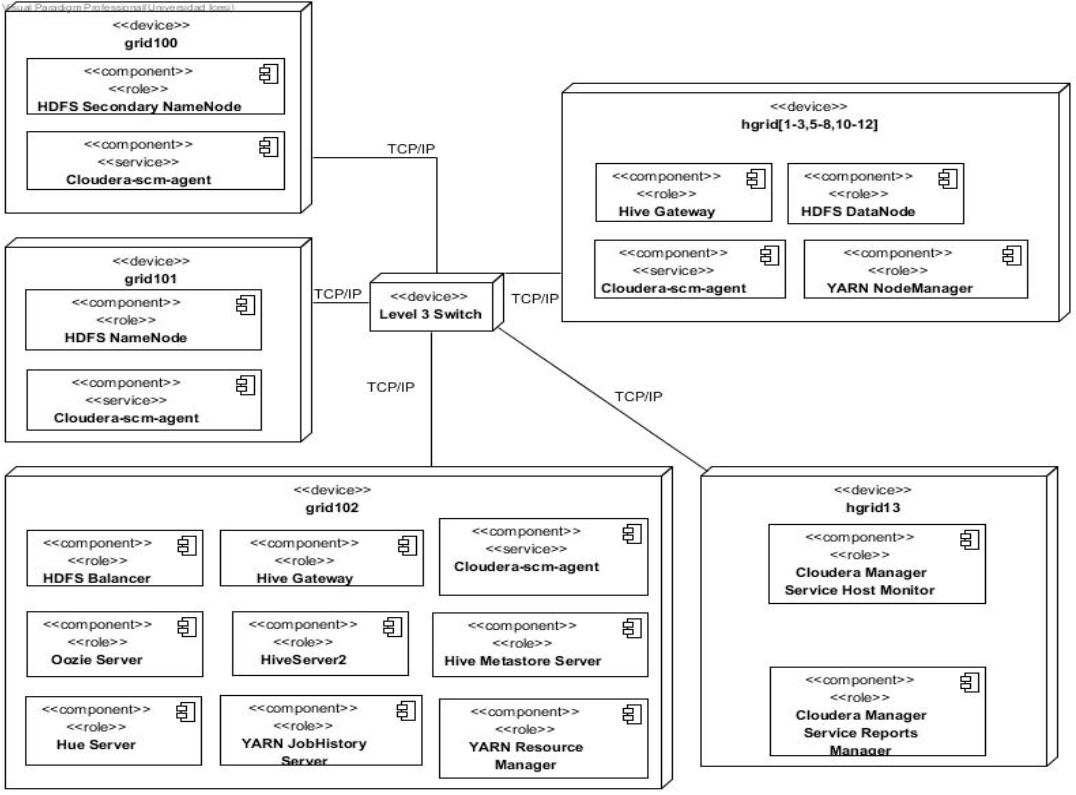
\includegraphics[width=6.0in, height=4.3in]{fig/deployment}
  \caption{Diagrama de despliegue de la configuración de CDH 5.10.1 en el laboratorio \textit{LIASON} de la Universidad Icesi.}
  \label{deployment_diagram}
\end{figure}

Cada uno de los casos de estudio de minería de datos presente en este proyecto se basa en los datos provistos por el \textit{National Climatic Data Center} (NCDC). Dichos datos son recolectados por medio de sensores climáticos, los cuales recolectan información cada hora, de forma diaria, en distintas estaciones a lo largo del mundo. Dichos datos se encuentran registrados a través de lineas en archivos de texto. La figura \ref{dataset} muestra la descripción del conjunto de datos mencionado previamente. \\

\begin{figure}[H]
  \centering
      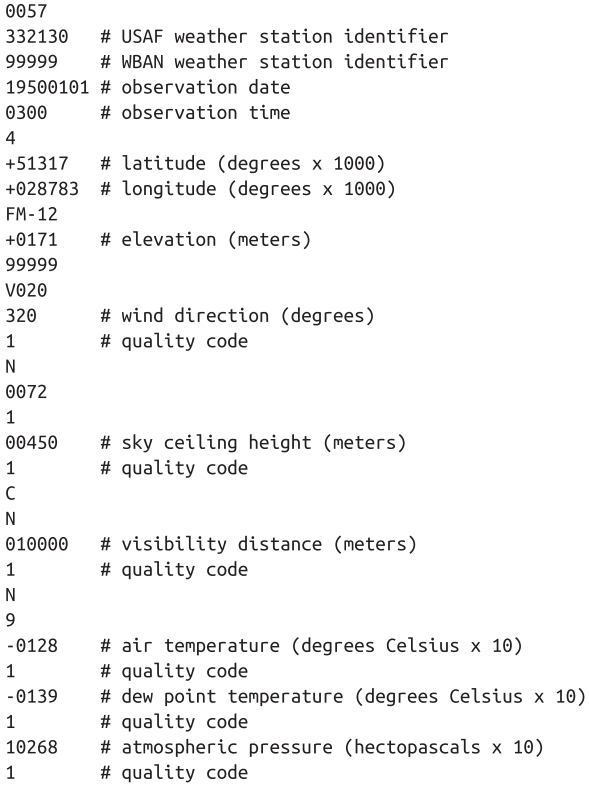
\includegraphics[width=5.0in, height=7.5in]{fig/dataset}
  \caption{Descripción del conjunto de datos. Tomado de \cite{White:2012:HDG:2285539}}
  \label{dataset}
\end{figure}

Vale la pena aclarar que en el presente documento se muestran los scripts y archivos de configuración más representativos de las distintas ejecuciones realizadas. Se omiten algunos elementos pues su contenido es muy similar a los ya presentados en este documento. Para una revisión más detallada de los distintos artefactos utilizados a lo largo de este proyecto, dirigirse a \url{https://github.com/lfrivera/Oozie-Pig-HCatalog-Demos}. Este repositorio contiene no solo el código fuente de las pruebas realizadas, sino también la evidencia (\textit{output} y \textit{screenshots}) de las mismas. \\

El resto del presente documento se encuentra distribuido como se muestra a continuación. En la sección 1 se describen formalmente el objetivo general y los objetivos objetivos específicos del proyecto. En la sección 2 se presentan los tipos de pruebas ejecutadas sobre las herramientas \textit{MapReduce}, \textit{Apache Pig}, y \textit{Apache Hive} para entender la diferencia entre los tiempos de ejecución de las mismas. En la sección 3 se presentan las pruebas ejecutadas para determinar la escalabilidad de Pig. En la sección 4 se ilustran las distintas pruebas llevadas a cabo sobre las herramientas \textit{Apache Pig} y \textit{HCatalog} para verificar la posibilidad de extender las funcionalidades y capacidades provistas por \textit{Pig}. En la sección 5 se detallan las pruebas realizadas sobre \textit{Apache Ooozie}, las cuales buscan evidenciar la reusabilidad y mantenibilidad de las aplicaciones desarrolladas sobre esta herramienta. La sección 6 muestra los resultados de la ejecución de las pruebas descritas previamente. En la sección 7 se presentan las conclusiones del presente trabajo. Finalmente, la sección 8 muestra las posibilidades de trabajo futuro que se podrían desarrollar a partir de lo que aquí se presenta.